\chapter{绪论}

\iffalse           %这是注释
\begin{figure}[htp]
	\centering
	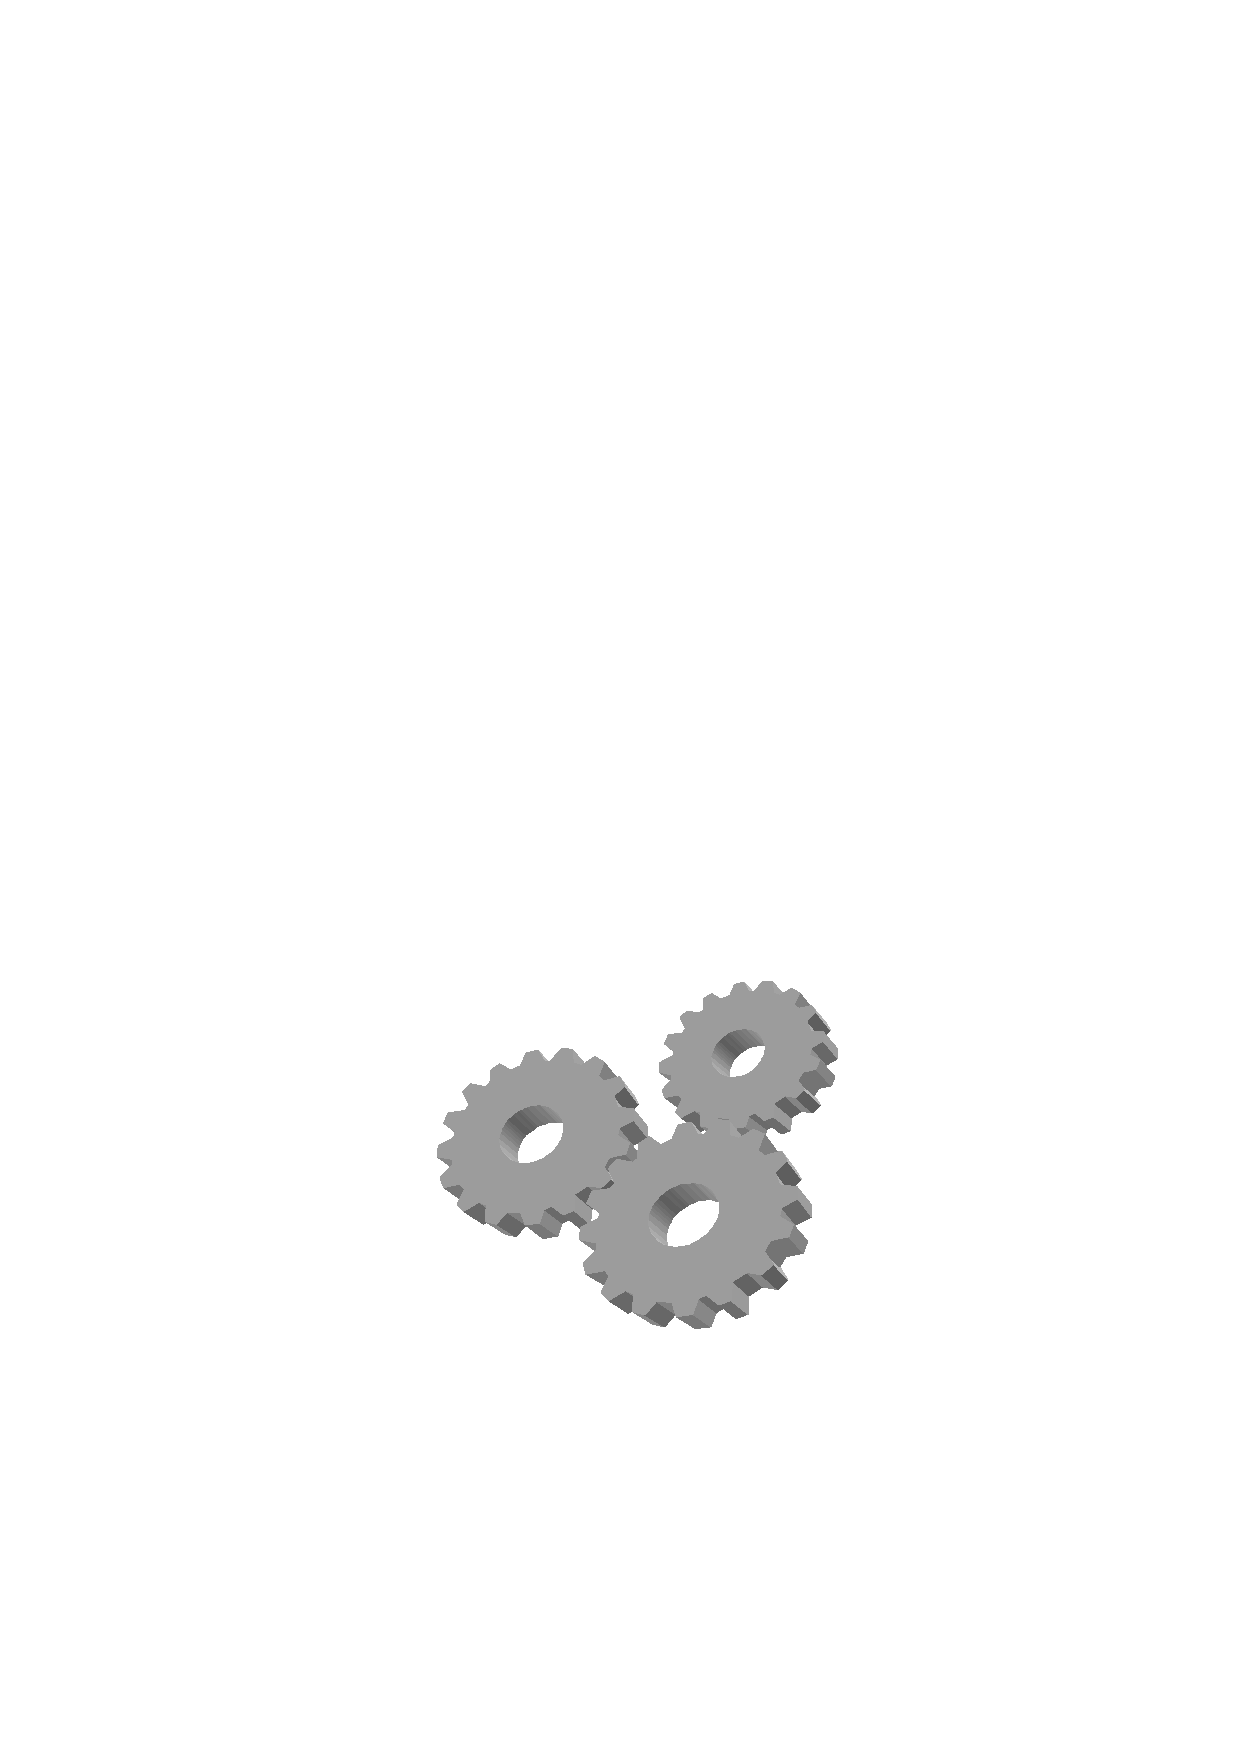
\includegraphics{picmain}
	\caption{图 1.1 名称}
\end{figure}

\begin{table}[htp]
	\centering
	\begin{minipage}[t]{0.8\linewidth} % 如果想在表格中使用脚注,minipage是个不错的办法
		\caption[表 1.1 名称]{}
		\begin{tabular*}{\textwidth}{lp{10cm}}
			\toprule[1.5pt]
			{\hei 列1} & {\hei 列2} \\
			\midrule[1pt]
			&  \\
			& \\
			& \\
			& \\
			& \\
			& \\
			\bottomrule[1.5pt]
		\end{tabular*}
	\end{minipage}
\end{table}


\cite{}

\fi



\section{研究背景与意义}


\subsection{研究背景}
地铁能够在短时间内运送大量乘客,从而减少城市拥堵、缓解地面交通压力,是现代城市交通的重要组成部分。
但是,受到公司运营成本、人员流动量大和人员流动速度较快等因素的限制,我国很多城市的地铁安检工作却较为宽松,并不能有效地防止爆炸物进入地铁环境。
爆炸事件一旦发生,将对地下丛横交错的城市水网、城市电网等公共设施造成破坏,
不仅会对疏散乘客和修复基础设施等工作带来诸多不便,危害公众的生命财产安全,还会对城市的高效运转和社会经济的快速发展产生巨大的不利影响。

传统的地铁排爆工作主要依赖排爆专家等技术人员深入爆炸环境排除爆炸物。然而,传统排爆方法却有很多弊端。
首先,爆炸物危害极大,一旦发生爆炸,将对排爆专家生命安全造成巨大危害。
其次,地铁内部的排椅和扶杆等结构化物体挤占了地铁内部空间,导致地铁内部空间较为狭窄。如果排爆专家身着排爆服进行排爆作业,空间移动将会收到很大限制。

随着智能机器人技术的快速发展,救援机器人在排爆领域逐渐开展应用。相比于传统排爆方法,救援机器人排爆展现出很多优势。
首先,救援机器人具有一定的自主能力,可以代替人类进入危险区域进行排爆作业,极大地降低了人员伤亡的风险。
其次,救援机器人体型较小便于在地铁排爆环境中移动,视角较低便于发现座椅下等隐匿的爆炸物,方便快速推进排爆工作。
再次,救援机器人可以携带多种传感器和设备,提高排爆的效率和准确性。

推动救援机器人在排爆环境中的自主作业,需要救援机器人感知周边环境。常见的传感器有激光雷达、RGB相机和RGB-D相机。
其中,激光雷达通过发射激光并捕捉物体表面反射的激光来生成高精度的三维点云数据。
但是,激光雷达一方面存在近距离盲区导致无法感知距离较近的物体,在狭窄的地铁环境中不利于感知环境。
另一方面,激光雷达获取环境数据稀疏,并且没有颜色信息和纹理信息。此外,激光雷达的成本也比较高。
RGB相机可以获取场景中物体丰富的颜色信息、形状信息和纹理信息,但是无法获取深度信息。
RGB-D相机集成了RGB相机和深度相机的功能。其中,RGB相机捕捉彩色图像,深度相机负责测量每个像素点到相机的距离,生成深度图像。
因此,RGB-D相机能够提供丰富的视觉信息,助力在狭窄的地铁环境中感知环境。

语义分割技术是地铁排爆场景语义理解的核心技术之一。相比于基于边框的目标检测而言,语义分割能够对场景进行更加精细和准确的解析。
语义分割通过通过给图像中的每个像素分配一个特定的类别,实现像素级图像理解。
通过像素级的图像理解,语义分割可以理解场景结构和布局,精确地识别和分类图像中的不同对象,为救援机器人在地铁排爆场景中的定位、建图、规划和决策等任务提供丰富的语义信息。

RGB-D语义分割的数据由彩色图像和对应的深度图像组合而成,两种图像虽然具有相同的数据结构,但是模态不同、数据内容不同,属于异质数据。
如何获取不同模态数据的有效信息、利用不同模态数据的互补性来提高语义分割的准确度是RGB-D语义分割的核心问题。
为了提升救援机器人感知系统的能力,本文的研究聚焦于RGB-D语义分割的异质数据特征提取与融合这个关键内容。


\subsection{研究意义}
本文的研究意义在于以下XX个方面:
(1)本文构建了一个地铁排爆场景的语义分割数据集,包括地铁闸机、楼梯、地铁内部常见物体以及模拟的管状爆炸物,覆盖了地铁场景从进站到乘车的几种常见场景。
(2)本文提出了一种XX方法。
(3)本文提出了一种XX方法。
(4)本文将上述两种算法应用到实际的救援机器人上,能够使救援机器人更好地理解地铁排爆场景,为救援工作的定位、建图、规划和决策提供丰富语义信息。
由此可见,本文的研究能为救援机器人提供可靠的语义信息,理解地铁排爆场景,进一步推动救援机器人全自主地铁排爆,具有较强的实际应用价值。


\section{国内外研究现状}

\subsection{三维传感器的研究现状}
相比于二维传感器而言,三维传感器可以捕获深度,获得场景的空间信息。常见的三维传感器主要包括激光雷达和RGB-D相机。
如\ref{图:常见的三维传感器} 所示。
\begin{figure}[h]
	\centering%
	\subfloat[激光雷达]{%
		\label{fig:rescue_1}
		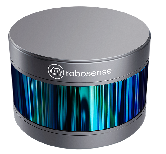
\includegraphics[width=0.15\textwidth]{figures/激光雷达.png}}
	\subfloat[双目深度相机]{%
		\label{fig:rescue_3}
		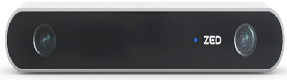
\includegraphics[width=0.25\textwidth]{figures/双目深度相机.png}}
	\subfloat[TOF深度相机]{%
		\label{fig:rescue_2}
		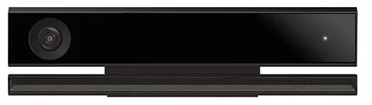
\includegraphics[width=0.25\textwidth]{figures/TOF深度相机.png}}
	\subfloat[结构光深度相机]{%
		\label{fig:rescue_4}
		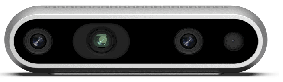
\includegraphics[width=0.25\textwidth]{figures/结构光深度相机.png}}
	\vspace{-1em}
	\caption{常见的三维传感器}
	\label{图:常见的三维传感器}
\end{figure}

在激光雷达中,由激光器发射出的脉冲激光在打到周围物体的表面时会发生反射,一部分反射激光会被激光雷达的接收器捕获,通过分析激光遇到目标对象后的在空中的折返时间,可以计算出激光雷达到目标对象的距离。
激光雷达通过从上到下逐层发射脉冲激光,得到目标对象上全部目标点的数据,比如空间坐标、反射率和表面纹理等,通过对这些数据进行成像处理,得到精准的三维点云图像。
根据成像原理,激光雷达有效探测距离可达上百米。但是激光雷达存在近距离盲区,无法捕捉自身周围1米内的物体信息。因此,激光雷达更适用于室外场景。


RGB-D相机整合了RGB相机和深度相机的优势,将两者集于一身。在获得彩色图像的同时,也获得了对应的深度信息,继而实现对周围环境的三维信息捕获。
深度相机的探测距离较短,但是近距离视野盲区半径可低至30厘米左右,相比于激光雷达,更适合在室内场景作业的机器人进行环境感知。


根据获取三维数据时是否主动发射出光波,RGB-D相机主要分为三种:被动式、主动式和多模态融合式。
依据这三种分类,发展出了不同的商用方案,主要有:双目视觉方案、飞行时间(Time of Flight, TOF)方案、结构光方案。

在双目视觉方案中,相机有两个类似人眼位置排列的RGB相机,利用这两个RGB相机获得不同位置得到的图像数据,基于图像特征点匹配原理对有视角差异的图像数据进行映射,通过计算图像特征点间的位置偏差,可以获取物体三维几何信息。
双目相机主要优点在于其硬件要求低,因此成本也低。
但是缺点也很明显。一方面,由于纯视觉方案对图像进行特征点的提取和匹配计算量大,因此对算法要求高,实时性效果较差。
另一方面,因为只有RGB一种传感器,对环境特征点的提取和匹配误差会较大,因此算法产生的深度精度不高。
如果场景特征不明显还会导致匹配失败,因此对纹理单调的场景不适用。
目前,双目深度相机在国外比较知名的生产商有:大疆,Intel, Stereolabs,Leap Motion等。


在飞行时间方案中,相机通过连续主动发射激光脉冲,再用传感器接收返回的激光脉冲,利用激光脉冲在空中的飞行时间来计算相机到目标物体的深度信息。
由于使用激光脉冲进行深度特测,因此TOF深度相机检测距离远,在激光能量充足的条件下可达几十米。
此外,激光脉冲在受环境光干扰的情况下,对成像效果影响较小。
但是,TOF深度相机的成本相对较高、体积较大。
目前,TOF深度相机在国外比较知名的生产商有:海康威视、联想、MicroSoft等。


在结构光方案中,相机通过近红外发射器,将具有一定结构特征的红外光线连续投影到目标三维空间的表面,然后基于接收模组收集并解析被物体表面反射回来的红外光线,得到物体的位置和深度信息。
因为,这种具备一定结构特征的红外光线会随着被摄物体深度的不同而产生不同的相位信息,运算单元可以将这种结构特征的变化换算成深度信息,并以此来获得三维结构。
结构光深度相机在近距离范围内精度和分辨率较高高,帧率可达60FPS。
但是,缺点也比较明显。
一方面,结构光容易受环境光干扰,室外成像效果比室内差。
另一方面,随检测距离增加精度会变差,因此,在远距离视野的精度较差。
目前,结构光深度相机在国外比较知名的生产商有:奥比中光,Apple,MicroSoft,Intel。


三种商用方案的粗略对比如\ref{表:深度相机性能对比} 所示。
\begin{table}[h]
	\caption{深度相机性能对比} % 标题
	\centering % 把表居中
	\renewcommand\arraystretch{1.2}
	\setlength{\tabcolsep}{16pt}
	\footnotesize
	\begin{tabular}{cccc} % 四个c代表该表一共四列,内容全部居中
		\toprule % 第一道横线
		相机类型     & 双目深度相机  & TOF深度相机 & 结构光深度相机 \\
		\midrule % 第二道横线 
		成像原理     & 双目特征匹配  & 飞行时间     & 激光散斑编码 \\
		\specialrule{0em}{1pt}{1pt} 
		分辨率       & 高           & 低          & 中 \\
		\specialrule{0em}{1pt}{1pt}
		成像精度     & 中           & 中          & 中 \\
		\specialrule{0em}{1pt}{1pt}
		制造成本     & 低           & 高          & 中 \\
		\bottomrule % 第三道横线
	\end{tabular}
	\label{表:深度相机性能对比}
\end{table}

通过对比以上三种方案可以看出,相比于双目视觉方案,结构光方案在环境适应性、近距离场景数据精度、实时性等方面表现较好;
相比于飞行时间方案,结构光方案的功耗更小,技术更成熟,制造成本更低。
因此,本文选择的传感器是Intel公司的Realsense系列的D435i,该款RGB-D相机采用结构光原理。






\subsection{传统的RGB-D语义分割}
传统的语义分割方法指不使用深度学习的方法。这种方法主要分为三个阶段。
在选择特征阶段,这类方法依赖手工设计的特征,比如颜色、纹理、形状等局部的外观属性,和一些局部特征描述子。
在分类输出阶段,将这些特征送入浅层机器学习分类模型,比如支持向量机(Support Vector Machine,SVM)和随机森林等,从而预测类别。
在结果优化阶段,用图模型,比如马尔可夫随机场(Markov Random Fields,MRF)和条件随机场(Conditional Random Fields,CRF),从而优化预测结果。


有一部分研究聚焦于手工特征的设计。
Shotton等人\cite{Shotton08CVPR}设计了一种新型低级特征语义纹理森林进行语义分割。
Scharwächter等人\cite{Scharwächter15IVS}联合处理了颜色、纹理和深度信息,通过随机决策森林快速推断出街景的粗略布局。


由于基于像素点的语义分割方法没有考虑像素与临近像素之间的关系,因此容易产生不一致的结果。
基于超像素的方法在一定程度上缓解了这个问题,该方法将在同一个局部区域中的像素强制预测成相同类别。
Gupta等人\cite{Gupta15IJCV}通过通用性和特异性特征来编码物体的外观和几何结构,将数据集中的超像素分类做为主要的物体类别,用随机森林和SVM分类,进一步提高了语义分割的准确性。


虽然基于超像素的方法对像素特征的提取更加鲁棒,但是超像素中的像素依然不能保持完全一致。概率图模型在一定程度上增强了空间一致性,从而缓解了这个问题。条件随机场提供一个概率框架,将输出间的关系描述为观测特征的函数。
Ladicky等人\cite{Ladicky10ECCV}针对CRF模型定义了一个全局能量函数,它结合了滑动窗口检测器的结果,以及基于像素的低水平一元和成对关系。
Cadena等人\cite{Cadena14ICRA}提出了一种有效的策略来诱导用于推理的CRF的图结构,增强了空间一致性。


传统的语义分割方法虽然取得了一些成果,但是人工设计的特征很难准确地表述复杂的场景环境,并且浅层机器学习分类模型对非线性函数的拟合能力有限。因此,针对较为复杂的分类问题,传统的语义分割方法效果很难提升。



\subsection{基于深度学习的RGB-D语义分割}
Hinton等人\cite{Hinton06Science}在2006年首次提出深度学习(Deep Learning,DL)之后,深度学习快速发展,语义分割研究也取得了突破性进展。与传统的语义分割方法相比,基于深度学习的语义分割方法能利用深度神经网络超强的非线性拟合能力,获取更多、更高级的语义信息来表达图像中的信息。


\subsubsection{基于卷积神经网络的RGB-D语义分割}
卷积神经网络(Convolutional Neural Network,CNN)的出现,极大地提升了语义分割地性能。
Long等人\cite{Long15CVPR}提出的全卷积神经网络(Fully Convolutional Network,FCN),第一次将深度神经网络引入语义分割领域。FCN推广了原有的CNN结构,利用特定的卷积层替换了常规卷积网络的全连接层,使得用于分类的CNN网络被转化为分割网络。
同时,利用转置卷积层实现上采样,使得网络可以执行密集推理并学习到图像中每个像素的语义标签。
此外,FCN可以处理任意大小的图像,语义分割速度也得到显著提升。
由于第一次实现了对图片进行端到端的训练,所以后续关于语义分割的研究几乎都借鉴了全卷积神经网络结构。

针对RGB-D双模态的语义分割, Couprie等人\cite{Couprie14MLR}提出了一种前融合方案。具体做法是将视频流逐帧分解,将彩色图片和深度图片拼连起来构成一个四通道的输入,放入卷积神经网络的四个输入,该方法实现了视频流的RGB-D实时语义分割,但是并没有区分不同模态的输入。
Gupta等人\cite{Gupta14ECCV}对深度数据进行编码为三个通道,包含水平视差(Horizontal disparity),地上高度(Height above groud)和重力夹角(the Angle the pixel’s local surface normal makes with the inferred gravity
direction)等信息,该编码结构加强了对深度信息的利用,但是不足在于需要相机的位姿等额外数据,并且编码计算代价较高。


















\iffalse 
上述策略都是围绕直接融合采集到的图片数据信息而提出的,即前融合策略, 但这类策略缺乏对不同模态数据的特征提取过程,通常无法兼具最优分割性能。

为了避免这一问题,Hazirbas等人在201 6年提出了一种基于双流网络进行间接特征融合的RGBD语义分割网络FuseNet[ 22],该方法设计了一种图像语义分割的编解码结构,通过在深度通道和图像通道之间添加中间特征映射,提升多模态数据的互补,获得了更好的融合效果。
同年,Li等人提出了一种新型(Long Short-Term Memorized Context Fusion,LSTM-CF)的网络模型[ 23],如图1.9所示,该方法通过水平和垂直多向融合实现全局上下文信息的整合,较好的利用了图像和深度的相关性,提高了语义分割的正确率。 


Long等人将其扩展到了RGB-D数据上:训练两个FCN网络,用来分别处理彩色图像和深度图像;再将两个网络的预测求和,得到最终的分类结果。为了提高融合的效率,Cheng等人设计了门控融合层来自动的学习高层的模态特异的特征[ 68]。
层次融合方法[ 66,71–74]可以在多个不同的层融合两个模态的特征。


FuseNet [71]以自底向上方式将多层的深度特征融入到RGB编码器。
RedNet[ 72]扩展了FuseNet,在自顶向下的路径上融合两个模态的多层特征。
SSMA[ 66]提出了一个自监督的模型适应融合机制(SSMA)来融合模态特征的特征,也是在自顶向下的路径上融合多层的特征。


例如,2017年Lee等人提出的RDFN et网络模型[ 24],就是基于当年里程碑式的RefineNet网络[ 25]而推广提出的。该网络较好的继承了残差学习机制, 通过MMFNet模块和多个RefineNet模块跳跃连接方式,细化图像和深度的融合方式,在试验验证中取得了较好的表现。

同年,Qi等人提出一种基于3D图网络的语义分割新网络模型3DGNN[26],通过将二维图像和深度信息融合,得到对应点的空间三维坐标(x,y,z),有效的减少了图片距离误导的错误发生,但在复杂场景或者二维/三维上下文相似场景中,也容易产生一定的误判。

同年,Schneider等人提出[ 27]了一种基于独立分支的RGBD中层特征融合模型,该方法具有较强的扩展性, 可通过简单的调整适用不同模态数据的处理,在公开数据集上保持了较高的性能指标。

针对深度几何信息在固定卷积神经网络上效果有限的问题,201 8年,Wang等人提出了深度感知卷积和深度感知平均池化[ 28]的算子,在不增加网络计算量的前提下,提高模型对两种模态数据的兼顾性,但实验结果表明这类方法对小目标的效果有限,需要在多尺度处理上进行改进。

同年,Jiang等人提出了一个对称的残差编解码网络[ 29],该网络深度很深却解决了细节遗失和梯度消失的问题,在小目标融合的效果上有显著提升。

近三年,基于深度学习的RGBD算法改进主要是针对语义特征提取网络的优化工作。
2019年Jiao等人提出了深度几何信息引入辅助语义分割的网络框架[ 30],该网络将骨干网络的权值相互分享,改进语义特征,并使用跳跃金字塔模块,提升上下文融合效果。

同年,Hu等人融入了注意力机制,提出了三平行分支架构的网络模型ACNet[ 3 1],充分融合深浅层特征,平衡图片和深度的作用比重,如图1.10 所示。

为了进一步充分利用两者互补性,在2020年北大、商汤科技、港大联合提出了一种引入作用于特征分离和聚合的注意力机制的网络模型[ 32],是互补信息重新校准融合。

2021年Chen等人提出的GLPNet网络[ 33]成功地在较深阶段保持两种信息稳定地传播,其原因在于引入局部上下文融合模块(L-CFM)进行动态对齐,引入全局上下文融合模块(G-CFM)进行联合建模。
\fi



 %\cite{Gupta14lECCV}





\subsubsection{基于transformer的RGB-D语义分割}


\subsubsection{基于mamba的RGB-D语义分割}





\section{主要研究内容与论文组织结构}


\subsection{主要研究内容}

\subsection{论文组织结构}




